%
See Fig. \ref{fig:3.8.1_speed}.  From the given information,  the rain velocity is
\begin{align}
\vec{u} = \myvec{0\\35}
\end{align}
%
and the wind velocity is 
\begin{align}
\vec{v} = -\myvec{12\\0}
\end{align}
%
The resulting rain velocity is 
\begin{align}
\vec{u}+\vec{v} = \myvec{-12\\35}
\end{align}
The desired angle is 
\begin{align}
-\tan^{-1}\phase{\vec{u}+\vec{v}} &= \tan^{-1}\frac{12}{35}
\\
&\approx 20.04 \degree
\end{align}  
%\begin{lstlisting}
%solutions/1/codes/line/speed.py
%\end{lstlisting}
\begin{figure}[!ht]
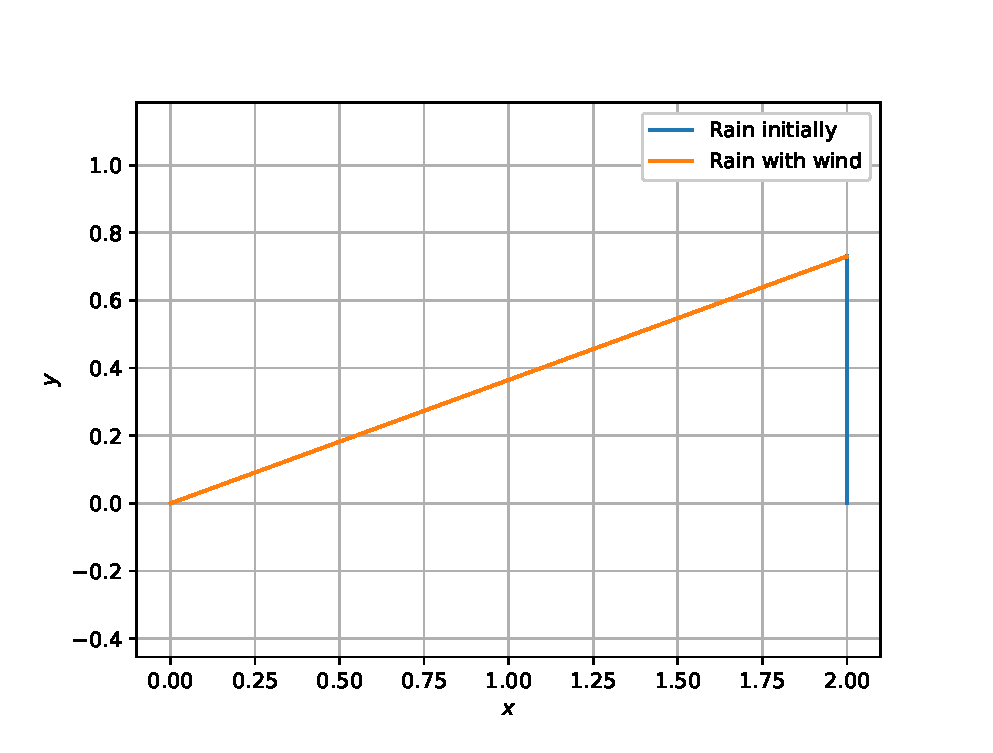
\includegraphics[width=\columnwidth]{./solutions/1/figs/line/speed.eps}
\caption{}
\label{fig:3.8.1_speed}
\end{figure}
